\begin{center}
  \centering
  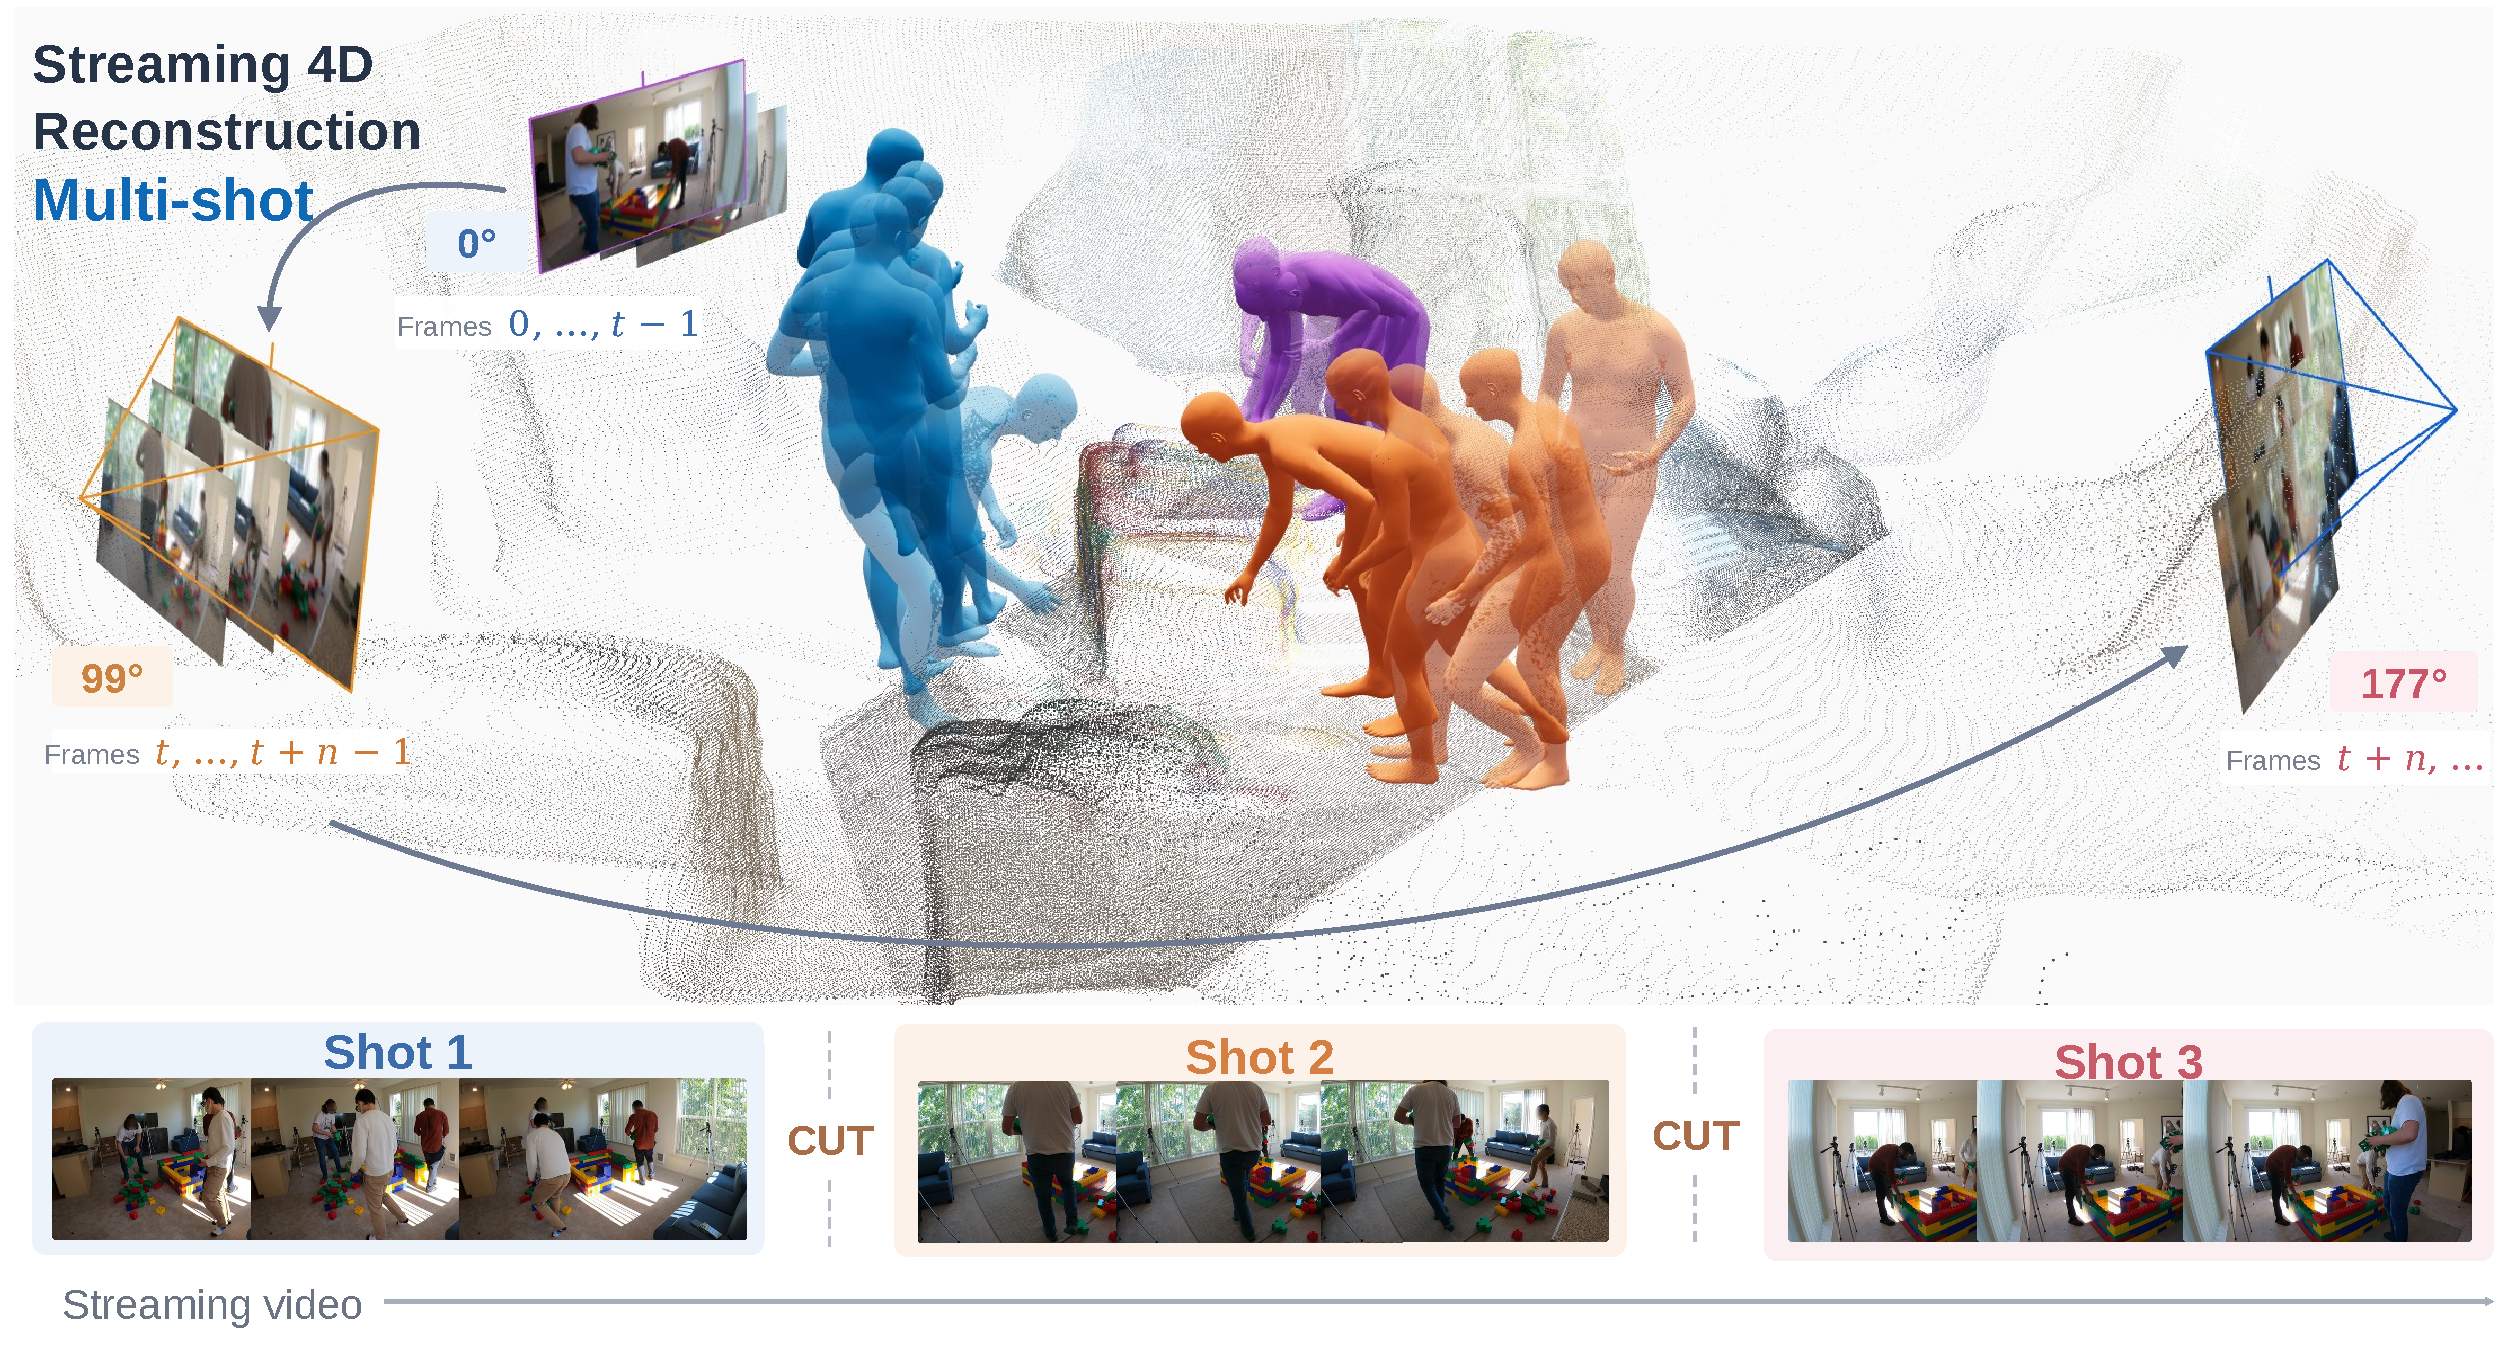
\includegraphics[width=0.86\textwidth]{figures/teaser.pdf}
  % 中文图注：三段按时间连接的单视角镜头及其共享世界坐标示意。上方和下方为输入帧，
  % 中央为示意性的世界坐标重建布局，并非模型输出的直接渲染；角度表示相对于第一镜头的
  % 源相机旋转。该图用于直观展示流式多镜头输入、镜头切换以及跨镜头的人体身份与空间一致性。
  % 图内标签中文：Streaming 4D Reconstruction=流式四维重建；Multi-shot=多镜头；Streaming video=流式视频；
  % Shot 1/2/3=镜头1/2/3；CUT=镜头切换；0/99/177 degrees=相对于第一镜头的源相机旋转角。
  \captionof{figure}{Shot3R streams successive monocular shots into a common
  world frame while preserving camera, motion, and identity continuity. Angles
  denote source-camera rotations from the first shot.}
  \label{fig:teaser}
\end{center}
